\section{Introduction} 

\paragraph{} %Intro générale
Volumetric objects are being more and more used in computer graphics.
They represent a volume by a function that associate a density to each point in world space.
This function can be defined analytically or with a dataset.
Since this representation does not contain topological information, volumetric objects are easy to manipulate.
They are hence a good candidate for procedural generation \cite{peytavie2009arches}.
They can be also be found in medical applications, considering they are the output of acquisition scanners.
Finally, this representation is widely used in gas and fluids simulation \cite{bridson2007fluid}.


\paragraph{} %Nos conditions pour assurer cette visualisation correcte
Visualising such objects is a crucial issue.
However, it imposes several constraints.
For interactive applications, it must be done in real-time.
We must also be able to render dynamic datasets such as fluids, as well as changing on the fly the data parameters.
Furthermore, visualising the results should be done as fast as possible to leave computational time for simulation purposes.
A solution would be to have a full GPU implementation that runs asynchronously from the CPU.
To sum up, an ideal method would fulfill those conditions:
\begin{itemize}
	\item Able to visualise volumetric objects in real-time.
	\item Able to handle dynamic datasets.
	\item Implemented entirely on the GPU.
\end{itemize}

\paragraph{}
There are two families of solutions to visualise volumetric data in real-time : ray casting and rasterization.
Ray casting  \cite{hadwiger2005real} accounts easily for lighting effects.
It also renders easily transparent surfaces, which can be useful when visualising medical datasets.
However, it does not fit the GPU pipeline and is thus slower than rasterization based solutions.

\paragraph{}
Our goal is to implement a solution that runs as fast as possible by taking full advantage of the GPU hardware. 
We thus choose to use rasterization.
This implies that a triangulated surface needs to be extracted from the data.
A very popular algorithm to do this triangulation is Marching Cubes (MC) \cite{lorensen1987marching}. 
It is data parallel so a GPU implementation of this method is very efficient \cite{tatarchuk2007real}.
During the rasterization process, each pixel of the framebuffer samples a unique triangle.
As a result, when several triangles project onto the same pixel, aliasing artefacts appear due to under-sampling (Figure \ref{lod}). 
To avoid such artefacts, the surface extraction must be adaptive to maintain a good sampling rate.

%\begin{figure}
%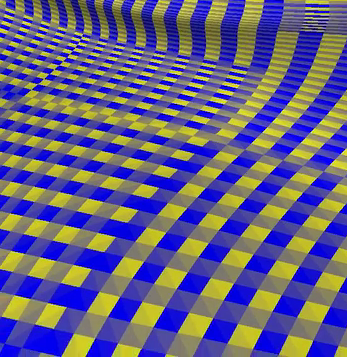
\includegraphics[height=0.125\textheight]{alias_close}
%\hfill
%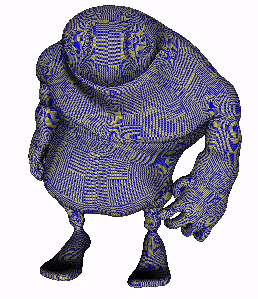
\includegraphics[height=0.125\textheight]{alias_far}
%\hfill
%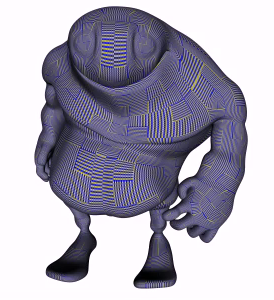
\includegraphics[height=0.125\textheight]{groundtruth}
%\caption{This model has a different color for each of its triangles. When close (Left), every triangle projects onto more than a pixel so the visualisation is fine. When viewed from distance (Middle), several triangles projects onto a single pixel and aliasing artefacts occur. (Right) is the same object visualised with 1024 samples per pixel.}
%\label{aliasing}
%\end{figure}

\paragraph{} %Situation par rapport au STAR
We are thus facing a problem of adaptive surface extraction, which is an extensively studied topic.
Many solutions have been developed in computational geometry \cite{shu1995adaptive,schaefer2004dual}.
However, they focus on the topology of the resulting mesh, whereas we focus on correct visualisation.
Real-time solutions have been developed using Level of Details (LoD). 
These methods dynamically refine the extracted triangulation using both the curvature of the object and its distance to the camera.
But since they rely on a preprocessing phase, they do not support visualising fully dynamic data in real-time.

\paragraph{}
Most of those LoD solutions were developed for heightfields visualisation \cite{duchaineau1997roaming}.
Yet, there are solutions that triangulate true volumetric data by applying MC on a hierarchical partition of space.
Since MC is not adaptive, the resulting hierarchical triangulation may carry cracks at resolution changes.
To avoid this, complex structures \cite{scholz2014real,schaefer2004dual} may be used or more triangles may be generated to stitch the holes \cite{lengyel2010voxel}.
Such adaptive methods run in real-time but they require both CPU and GPU time.
Furthermore, for performance purposes, some of them cache parts of the triangulation, which prevents the use of fully dynamic data.
Finally, none of the aforementioned solutions ensure a minimal triangle size, and are thus subject to aliasing issues.

\paragraph{} %What we do
The method developed by Lengyel \textit{et al.} \cite{lengyel2010voxel} is the best suited to our needs.
However, it was preferably developed to visualise in real-time static or near static data and present a complex CPU implementation.
In this paper we propose a GPU pipeline inspired from this method.
It leaves the CPU free for other tasks and avoids synchronisation with the GPU.
Our high framerate also allows this method to run in real-time on fully dynamic data. 
The triangulation is controlled by a GPU LoD criterion that ensures that triangles project onto more than one pixel, thus removing geometrical aliasing.

\paragraph{}
In the next section, we present the main algorithms on which our work is based \cite{lengyel2010voxel,dupuy2014quadtrees}. 
Then, we present our GPU implementation, followed by our results and performances.
Finally, we end up by concluding on the limitations and perspectives of our approach.
